\chapter{Výsledky}

V této kapitole prezentujeme výsledky vybraných architektur z kapitoly \hyperref[chap:experimenty]{Experimenty} na testovacích datech a provádíme kvantitativní a kvalitativní srovnání se state-of-the-art systémy pro extrakci melodie, představené v kapitole \hyperref[chap:souvisejici]{Související práce}.

\section{Výběr testovaných modelů}

Pro srovnání jsme vybrali nejlepší modely od každé testované architektury, pomocí provedených experimentů prezentujeme v tabulkách pro každou architekturu nejlepší nalezené nastavení hyperparametrů.

\subsection{Architektura CREPE}

Zvolený model dosáhl na validačních datech přesnosti přepisu výšky 0.689 a přesnosti přepisu výšky nezávisle na oktávě 0.784. Počet trénovatelných parametrů tohoto modelu je $7\,816\,640$, trénovaní probíhalo téměř 9 hodin, každý trénovací příklad byl síti předložen 10 krát (proběhlo 10 epoch trénování).

\begin{table}[h!]
\begin{tabular}{llll}
\hline
\toprule
Prohledávané parametry               &          & Ostatní parametry &         \\
Parametr                             & Hodnota  & Parametr          & Hodnota \\
\midrule
Multiplikační koef. kapacity         & 16       & Velikost dávky    & 32      \\
Rozlišení diskretizace výšky noty    & 5        & Iterace trénování & 360000  \\
Rozptyl distribuce výšky noty & 0.177    & Learning rate     & 0.001   \\
Šířka vstupního okna                 & 4096     &                   &         \\
Násobné rozlišení první vrstvy       & 6 vrstev &                   &         \\
\bottomrule
\end{tabular}
\end{table}

\subsection{Architektura WaveNet}

\textcolor{red}{TODO vybrat}

\subsection{Architektura HCNN}

\textcolor{red}{TODO dotrénovat nějaký lol}

\subsection{Architektura pro detekci melodie}

- modul detekce melodie bude mít k dispozici výstup HCNN

\section{Kvantitativní srovnání}

\textcolor{red}{Tohle je tak trochu placeholder, protože ještě čekám na nějaká čísla}

\begin{table}[h!]
\centering

\begin{tabular}{lrrrrrr}
\toprule
              Metoda & ADC04 & \shortstack[r]{MDB-mel-s \\ test} & \shortstack[r]{MIREX05\\train.} & \shortstack[r]{MDB\\test} & ORCHSET & \shortstack[r]{WJazzD\\test} \\
\midrule
        Salamon & 0.767 &                 0.514 &          0.761 &         0.526 &   0.281 &       0.693 \\
        Bittner & 0.814 &                 0.606 &          0.807 &         0.670 &   0.519 &       0.774 \\
        Basaran & 0.793 &                 0.733 &          0.798 &         0.706 &   0.635 &       0.767 \\
          CREPE & 0.793 &                 0.542 &          0.783 &         0.607 &   0.395 &       0.784 \\
        WaveNet & 0.799 &                 0.532 &          0.790 &         0.595 &   0.363 &       0.761 \\
  \shortstack[r]{Bittner\\Improved} & 0.856 &                 0.707 &          0.855 &         0.734 &   0.595 &       0.806 \\
\bottomrule
\end{tabular}

\caption{Výsledky přesnosti přepisu (Raw Pitch Accuracy).}\label{tab:vysledky_RPA}
\end{table}

\begin{table}[h!]
\centering

\begin{tabular}{lrrrrrr}
\toprule
              Metoda & ADC04 & \shortstack[r]{MDB-mel-s \\ test} & \shortstack[r]{MIREX05\\train.} & \shortstack[r]{MDB\\test} & ORCHSET & \shortstack[r]{WJazzD\\test} \\
\midrule
        Salamon & 0.807 &                 0.639 &          0.805 &         0.659 &   0.568 &       0.757 \\
        Bittner & 0.855 &                 0.666 &          0.824 &         0.735 &   0.694 &       0.785 \\
        Basaran & 0.820 &                 0.766 &          0.807 &         0.757 &   0.776 &       0.776 \\
          CREPE & 0.853 &                 0.614 &          0.817 &         0.713 &   0.606 &       0.810 \\
        WaveNet & 0.850 &                 0.604 &          0.826 &         0.706 &   0.573 &       0.796 \\
 \shortstack[r]{Bittner\\Improved}   & 0.894 &                 0.746 &          0.872 &         0.787 &   0.762 &       0.815 \\
\bottomrule
\end{tabular}

\caption{Výsledky přesnosti přepisu nezávisle na oktávě (Raw Chroma Accuracy).}\label{tab:vysledky_RCA}
\end{table}

\section{Kvalitativní srovnání}

- celkově moc není příklad, na kterém je HCNN výrazně lepší než obě metody (krom train10 mirex)
- Basaran je horší v jazzu kvůli kvantifikaci
- zase je lepší v orchsetu kvůli lepší vstupní reprezentaci
- 

Pro srovnání sítí na jednotlivých příkladech jsme vybrali na základě kvantitativního vyhodnocení metody Bittnerové a Basarana. Z testovaných architektur vybíráme HCNN, jelikož výsledky této metody v přepisu melodie předčily stávající metody na většině testovacích datasetů. Pro srovnání vybíráme příklady, ve kterých se výstupy sítí nejvíce lišily.

\begin{figure}[h]\centering
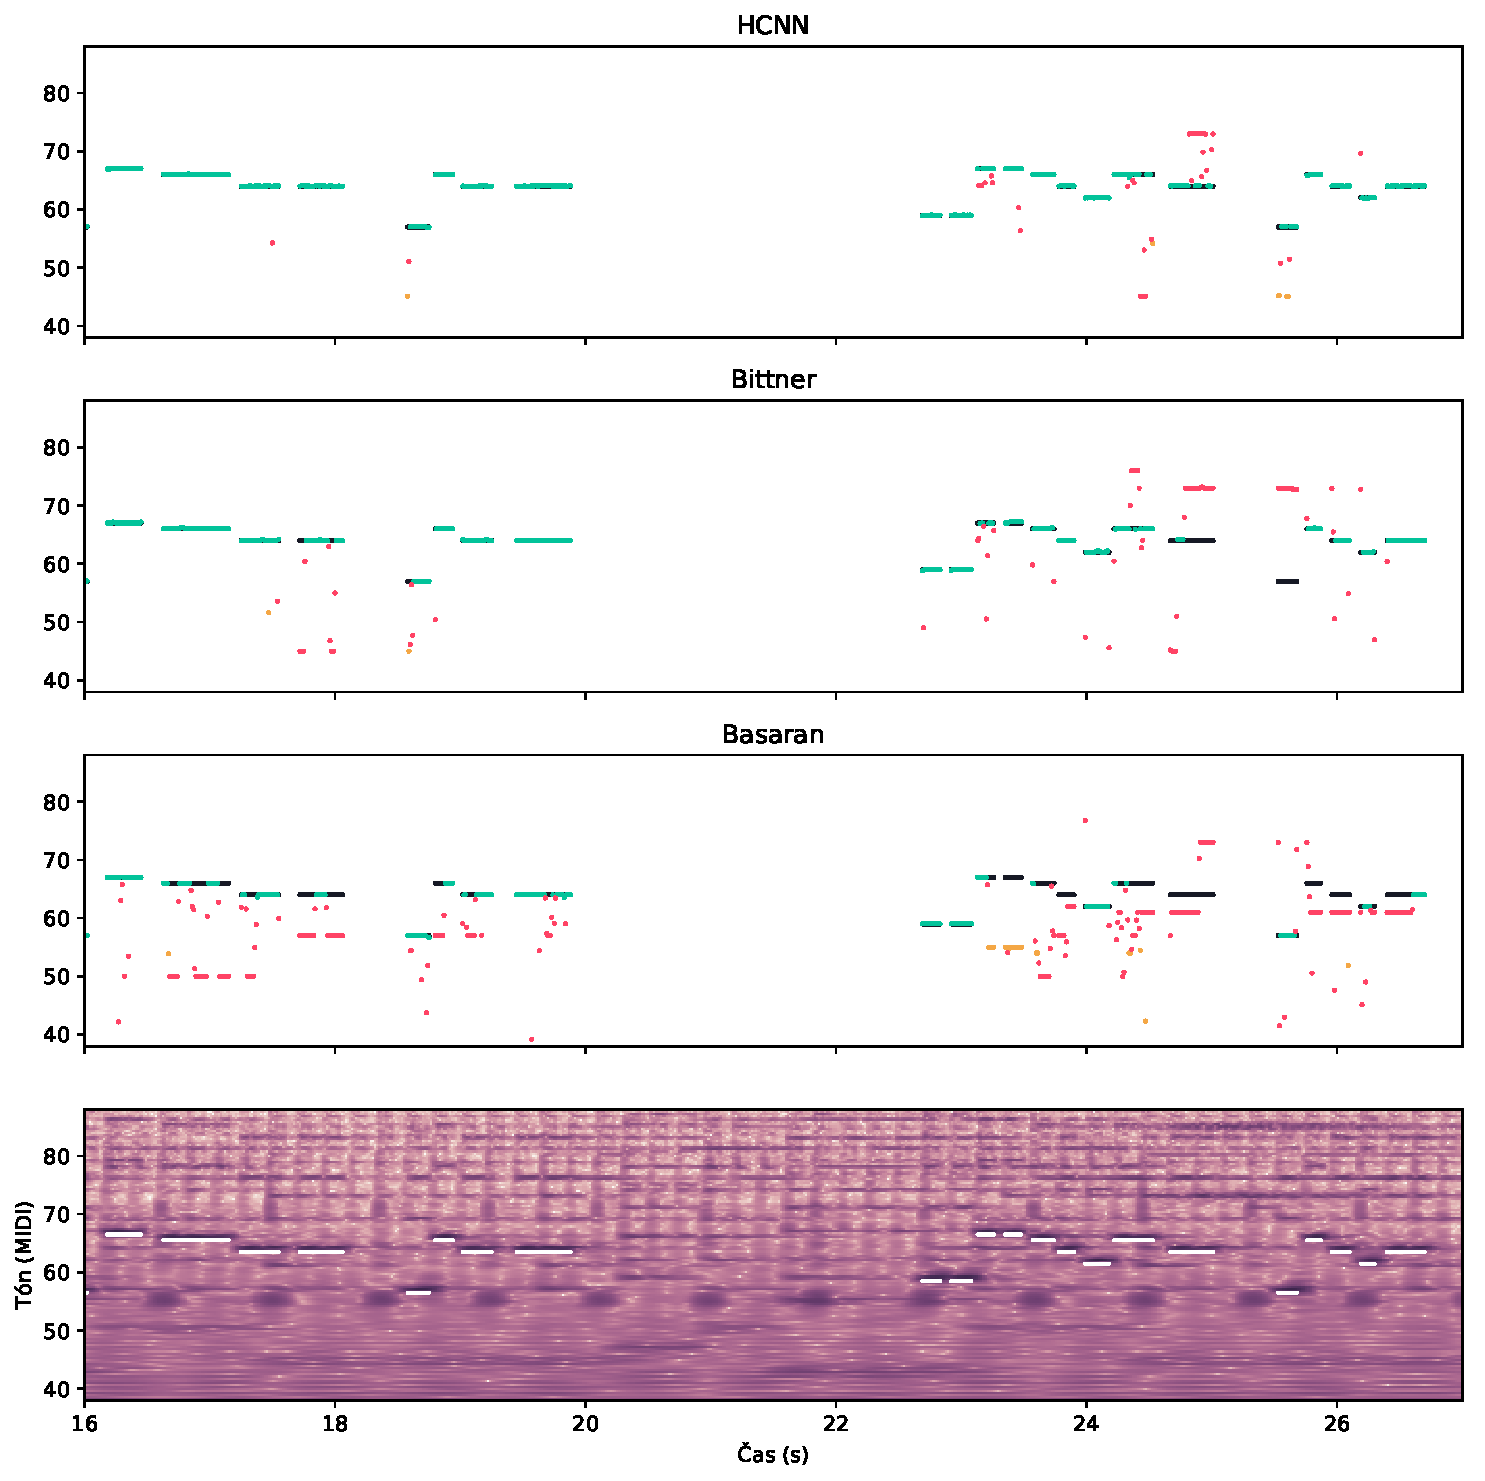
\includegraphics[width=\textwidth,height=\textheight,keepaspectratio]{../img/vysledky/mirex05_train10}
\caption{Výstup metod na testovacím souboru \texttt{train10} z datasetu MIREX05.}
\label{obr:mirex05_train10}
\end{figure}

\begin{figure}[h]\centering
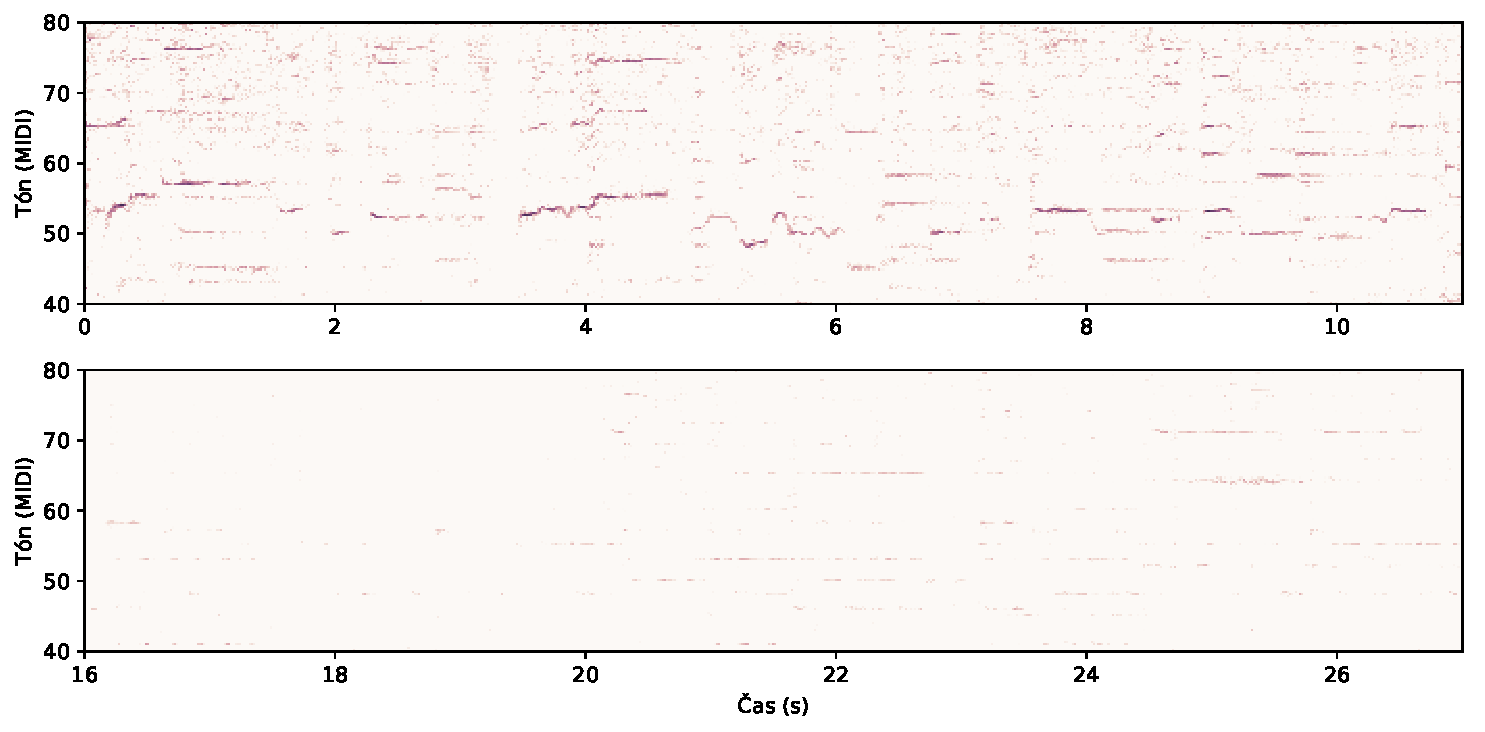
\includegraphics[width=\textwidth,height=\textheight,keepaspectratio]{../img/vysledky/basaran_salience_comparison}
\caption{Srovnání vstupní frekvenčně-časové reprezentace $\bm{\mathrm{H}}^{F_0}$ Basaranovy metody testovacích souborů \texttt{train01} a \texttt{train10} z datasetu MIREX05.}
\label{obr:basaran_salience_comparison}
\end{figure}

\begin{table}[h]
\centering

    \begin{tabular}{ll}
    \toprule
    Metrika (Metoda) & train10 \\
    \midrule
          RPA (HCNN) &   0.917 \\
          RCA (HCNN) &   0.934 \\
      RPA (Bittner) &   0.863 \\
      RCA (Bittner) &   0.868 \\
      RPA (Basaran) &   0.512 \\
      RCA (Basaran) &   0.572 \\
    \bottomrule
    \end{tabular}

\caption{Přesnost metod na testovacím souboru \texttt{train10} z datasetu MIREX05.}\label{tab:mirex05_train10}
\end{table}

Největší slabinou sítě HCNN se stala podle očekávání časová kontinuita odhadů. Protože síť pro odhad výšek uvažuje vždy pouze $5.8\,\rm ms$ a po vytvoření funkce salience na odhady tónů neaplikujeme žádné způsoby vyhlazování, odhady jednotlivých časových oken na sebe nenavazují. To se nejeví jako zásadní problém v případech, kdy ve skladbě melodii nenese více hlasů v souzvuku (viz výstup \ref{obr:mirex05_train10}). U některých orchestrálních skladeb však vzniká problém, například pokud melodii nese zároveň sekce smyčců a dechů v různých oktávách. Jak můžeme vidět na výstupu algoritmů \ref{obr:orchset_Musorgski-Ravel-PicturesExhibition-ex6}, HCNN pak \uv{přeskakuje} mezi oktávami. Problém je také dobře vidět na výstupní funkci salience \ref{obr:orchset_Musorgski-Ravel-PicturesExhibition-ex6_salience}, na které vidíme tři totožné kontury posunuté o oktávu. Mírné zlepšení tohoto problému vidíme na výstupech metody \cite{Bittner2017}, která podobně jako naše metoda výsledek funkce salience žádným způsobem nezpracovává, na druhou stranu její metoda pro odhad výšky uvažuje okno délky $150\,\rm ms$. Na obrázku \ref{obr:orchset_Musorgski-Ravel-PicturesExhibition-ex6} vidíme, že množství oktávových chyb je výrazně menší --- díky většímu kontextu může metoda vybrat v čase navazující odhady. Metoda týmu \cite{DBasaranSEssid2018} odhad výšky tónů vyhlazuje pomocí rekurentní architektury GRU, tudíž jejich výstup obsahuje nejméně skoků. Použití rekurentní sítě dovoluje zachytit ještě dlouhodobější závislosti a výstupní kontura pak jednak často obsahuje nejmenší množství velmi krátkých, chybných skoků mimo hlavní melodii, které se na obrázku \ref{obr:orchset_Musorgski-Ravel-PicturesExhibition-ex6} hojně vyskytují u metod bez vyhlazování a jednak je celkový průběh výsledné kontury často koherentnější. Další výraznou slabinu jsme z analýzy jednotlivých výstupů sítí neregistrovali. U výstupů, ve kterých se sítě nejvíce lišily, byl tento rozdíl nejčastěji způsoben právě těmito diskontinuitami, případně pak zachycením jiného než hlavního nástroje v pozadí. Největší rozdíly ve výsledcích jsou proto na datasetu ORCHSET, ve kterém je výskyt polyfonie nejčastější. 

\begin{figure}[h]\centering
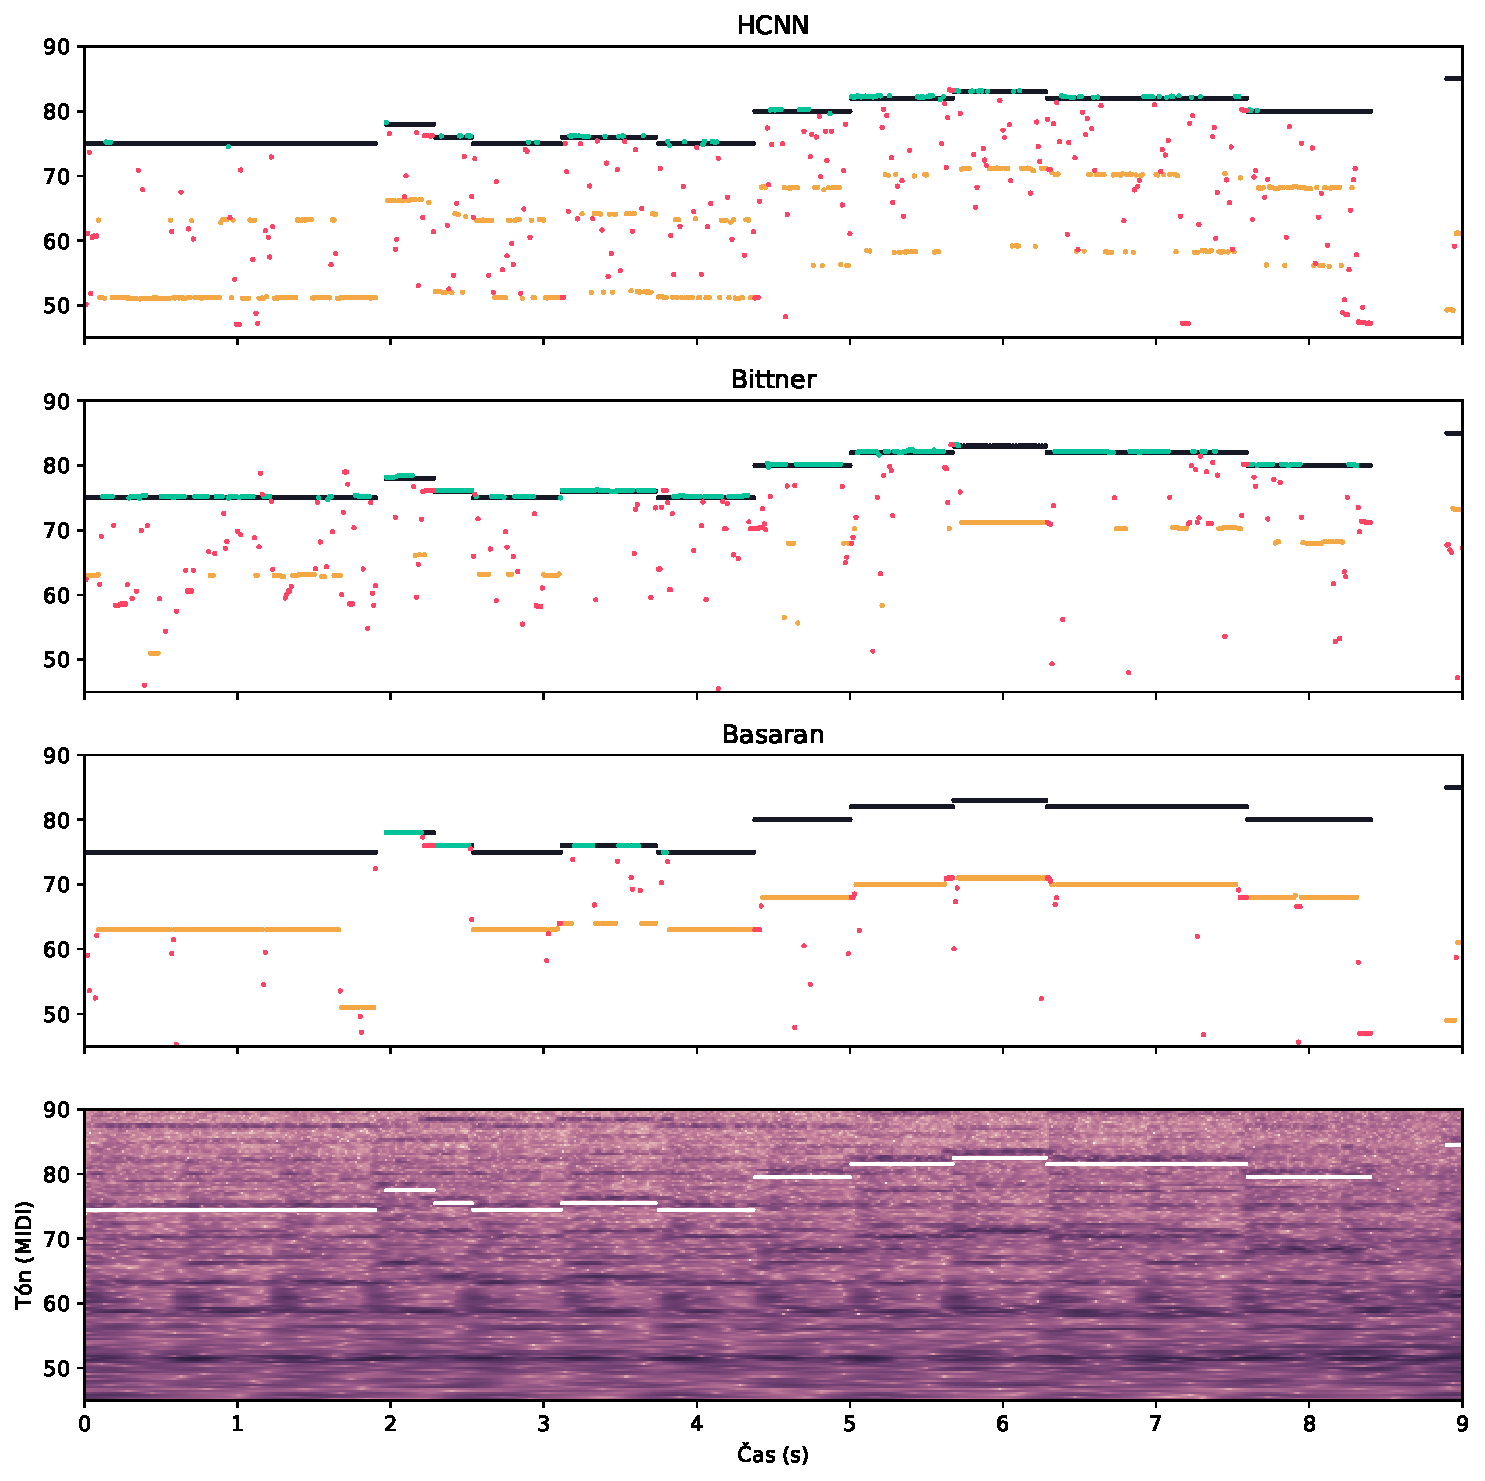
\includegraphics[width=\textwidth,height=\textheight,keepaspectratio]{../img/vysledky/orchset_Musorgski-Ravel-PicturesExhibition-ex6}
\caption{Výstup metod na testovacím souboru \texttt{Musorgski-Ravel-PicturesExhibition-ex6} z datasetu ORCHSET.}
\label{obr:orchset_Musorgski-Ravel-PicturesExhibition-ex6}
\end{figure}

\begin{table}[h]
\centering

    \begin{tabular}{ll}
    \toprule
    Metrika (Metoda) & Musorgski-Ravel-PicturesExhibition-ex6 \\
    \midrule
          RPA (HCNN) &                                  0.125 \\
          RCA (HCNN) &                                  0.725 \\
      RPA (Bittner) &                                  0.397 \\
      RCA (Bittner) &                                  0.826 \\
      RPA (Basaran) &                                  0.040 \\
      RCA (Basaran) &                                  0.914 \\
    \bottomrule
    \end{tabular}

\caption{Přesnost metod na testovacím souboru \texttt{Musorgski-Ravel-PicturesExhibition-ex6} z datasetu ORCHSET.}\label{tab:orchset_Musorgski-Ravel-PicturesExhibition-ex6}
\end{table}

\begin{figure}[h]\centering
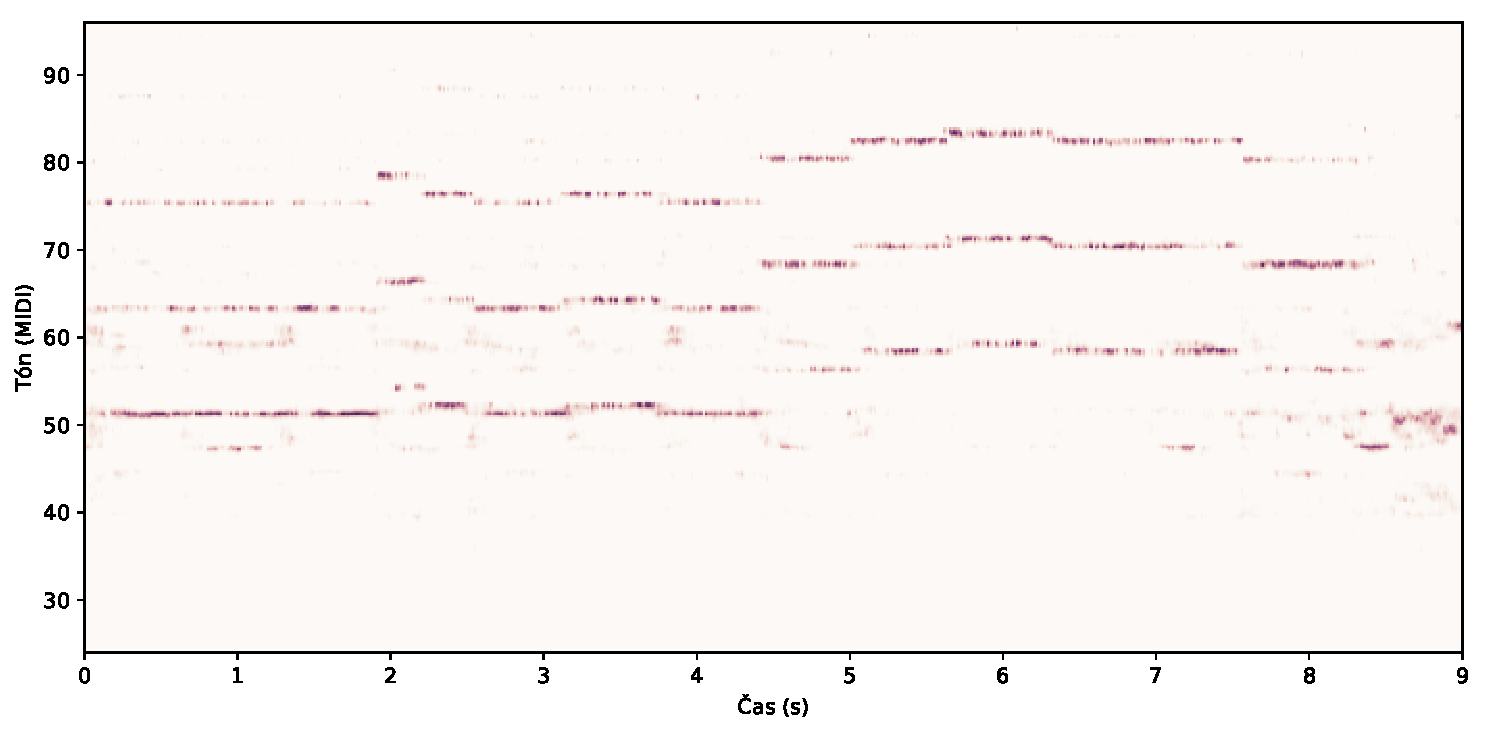
\includegraphics[width=\textwidth,height=\textheight,keepaspectratio]{../img/vysledky/orchset_Musorgski-Ravel-PicturesExhibition-ex6_salience}
\caption{Výstupní salience metody HCNN na testovacím souboru \texttt{Musorgski-Ravel-PicturesExhibition-ex6} z datasetu ORCHSET.}
\label{obr:orchset_Musorgski-Ravel-PicturesExhibition-ex6_salience}
\end{figure}

Basaranova metoda pro tuto kontinuitu tónů však obětovala přesné znějící výšky tónů. Jak jsme již prezentovali v kapitole Experimenty, výstup metod kvantizovaný na půltóny obsahuje množství chyb, jelikož často selhává v zachycení frekvenčních modulací. Na obrázku \ref{obr:wjazzd_CannonballAdderley_SoWhat_detail} vidíme další limitaci takového výstupu --- pokud je obsah skladby laděný podle jiného referenčního tónu než jaký byl použit pro trénování sítě, znějící tóny vycházejí výškou \uv{mezi} výstupní složky. Z tabulky \ref{tab:wjazzd_CannonballAdderley_SoWhat} a obrázku \ref{obr:wjazzd_CannonballAdderley_SoWhat} je pak zřejmé, že kvůli této kvantizaci síť nedosahuje srovnatelných výsledků, přestože na jiných, žánrově shodných datech, které jsou laděny na správný referenční tón, podává kompetitivní výsledky. Limitace se proto týká zejména jazzových nahrávek pocházejících z období před rokem 1955, před zavedením referenčního tón A4=440Hz ve standardu ISO16.


\begin{figure}[h]\centering
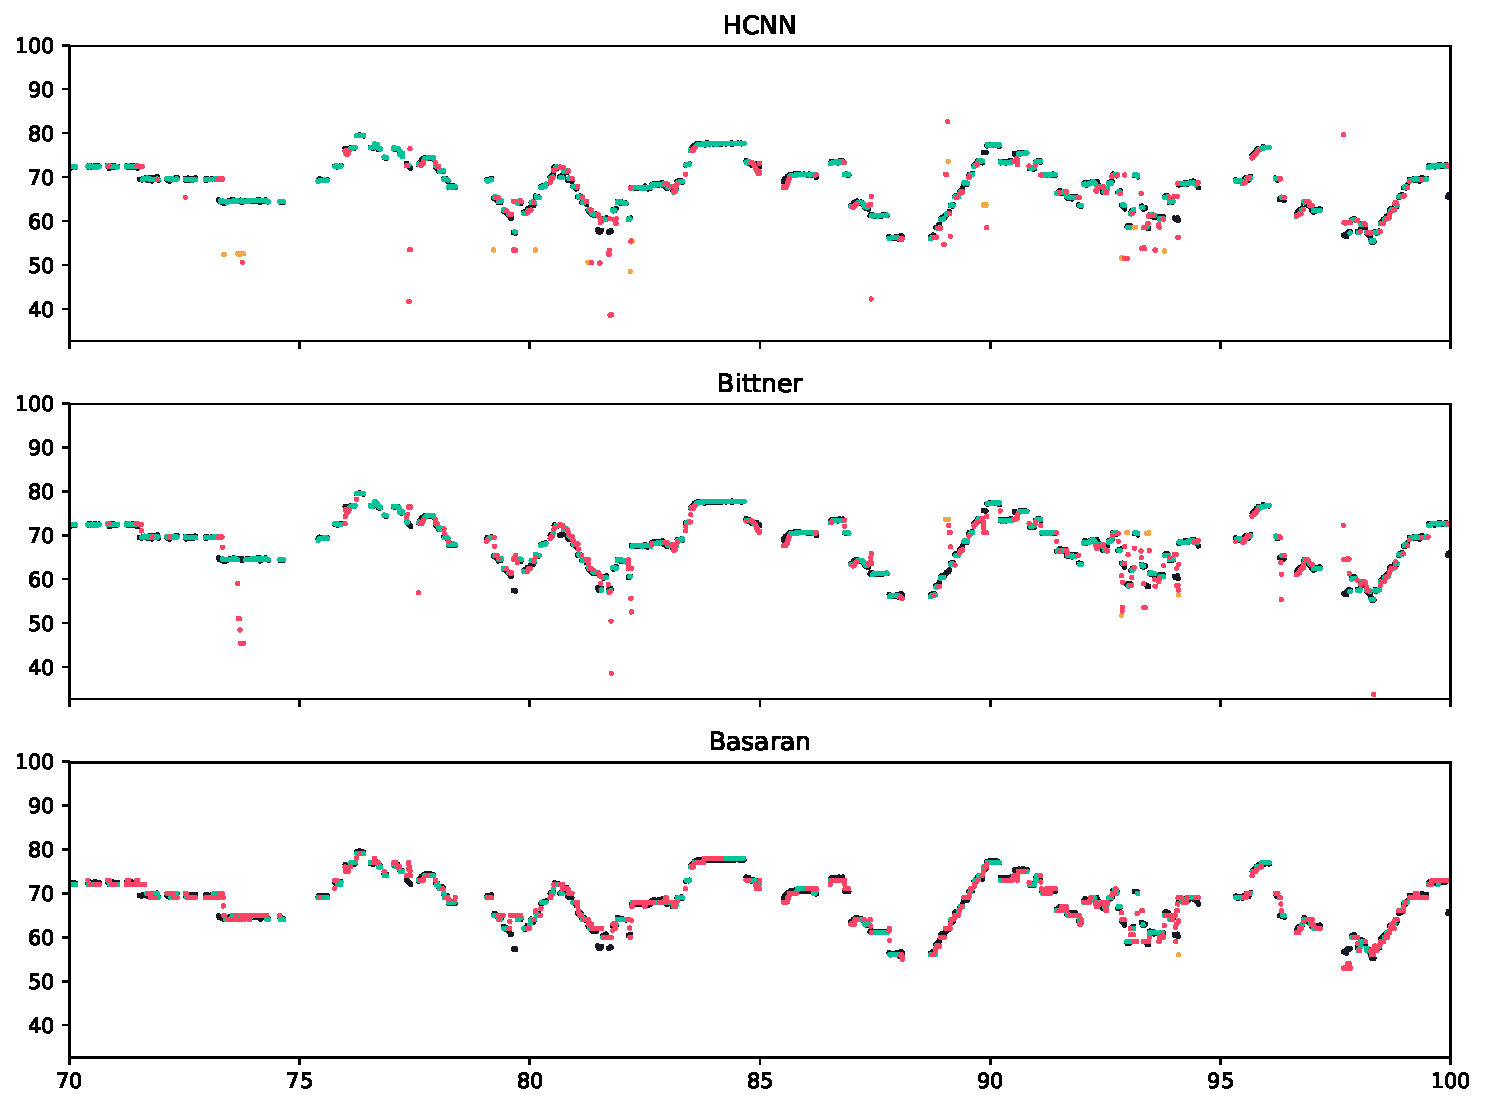
\includegraphics[width=\textwidth,height=\textheight,keepaspectratio]{../img/vysledky/wjazzd_CannonballAdderley_SoWhat}
\caption{Výstup metod na testovacím souboru \texttt{CannonballAdderley\_SoWhat} z datasetu WJazzD.}
\label{obr:wjazzd_CannonballAdderley_SoWhat}
\end{figure}

\begin{table}[h]
\centering

\begin{tabular}{ll}
\toprule
Metrika (Metoda) & CannonballAdderley\_SoWhat \\
\midrule
      RPA (HCNN) &                     0.850 \\
      RCA (HCNN) &                     0.861 \\
   RPA (Bittner) &                     0.828 \\
   RCA (Bittner) &                     0.833 \\
   RPA (Basaran) &                     0.653 \\
   RCA (Basaran) &                     0.656 \\
\bottomrule
\end{tabular}

\caption{Přesnost metod na testovacím souboru \texttt{CannonballAdderley\_SoWhat} z datasetu WJazzD.}\label{tab:wjazzd_CannonballAdderley_SoWhat}
\end{table}


\begin{figure}[h]\centering
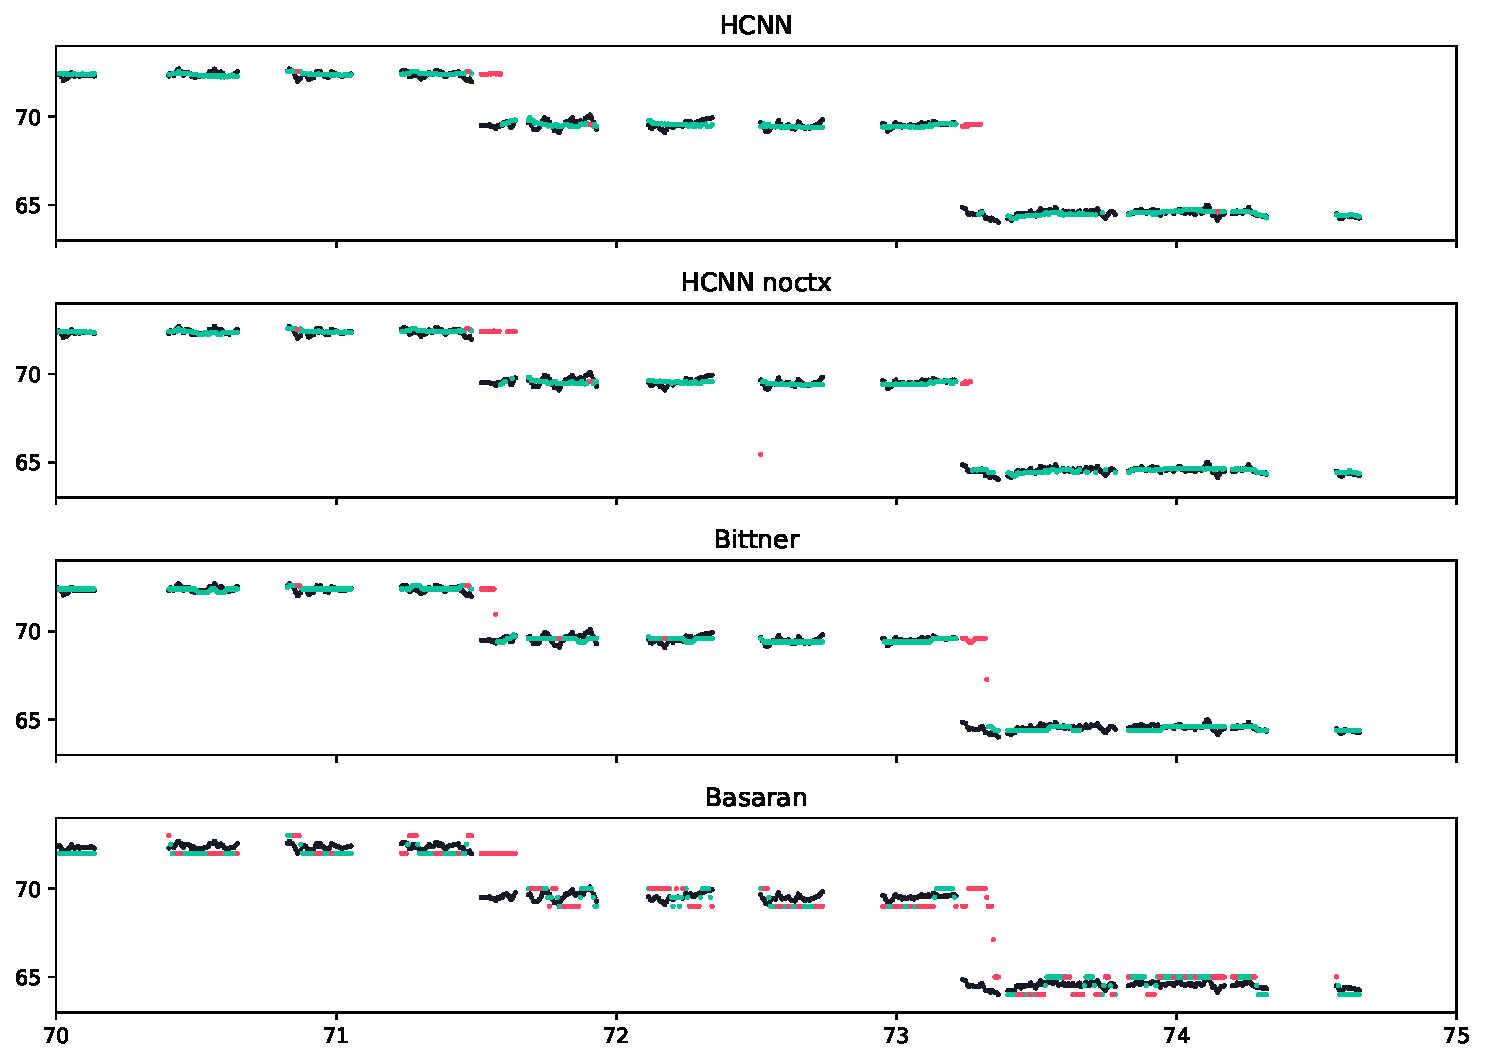
\includegraphics[width=\textwidth,height=\textheight,keepaspectratio]{../img/vysledky/wjazzd_CannonballAdderley_SoWh}
\caption{Detail přepisu metod na testovacím souboru \texttt{CannonballAdderley\_SoWhat} z datasetu WJazzD.}
\label{obr:wjazzd_CannonballAdderley_SoWhat_detail}
\end{figure}


Dalším problémem Basaranovy metody je zhoršená schopnost extrakce na syntetických datech. Příklady \texttt{midi2REF}, \texttt{midi3REF}, \texttt{train10REF} z datasetů ADC04 a MIREX05 jsou syntetizovány na základě MIDI pomocí základních zvukových fontů, nahrávky proto zní velmi uměle. Jak vidíme na obrázku \ref{obr:mirex05_train10}, zatímco metody Bittnerové a HCNN si s touto syntetickou barvou hlasu dokáží poradit, výstup Basaranovy metody obsahuje šum a skoky k doprovázejícím nástrojům. Příčinou může být jiná vstupní reprezentace signálu, která je založena na práci \cite{Durrieu2010} a spočívá na modelování hlavního hlasu pomocí zdroje a filtrů. Na obrázku \ref{obr:basaran_salience_comparison} srovnáváme tuto reprezentaci pro vstupní signál s lidským zpěvem (nahoře, \texttt{train01}) a pro signál se syntetickou flétnou (dole, \texttt{train10}). Je zřejmé, že zatímco lidský zpěv tato reprezntace dokáže zachytit, syntetický hlas na reprezentaci téměř zachycen není. 

Rozdílem mezi HCNN a metodou Bittnerové jsou zejména jiné priority, které přiřazují barvám hlasů, lze tudíž nalézt mnoho příkladů, kde HCNN zároveň přepisuje melodii a nesprávně místy přeskakuje nástroji v doprovodu, zatímco metoda Bittnerové na stejném příkladu tuto chybu nedělá. Podobně existují i opačné příklady. Zajímavým případem je soubor \texttt{MatthewEntwistle\_FairerHopes} z kolekce MedleyDB, ve kterém melodii hraje harfa, která se však nevyskytuje v množině trénovacích dat. Zatímco metoda HCNN zvládá generalizovat i na dosud neslyšené barvy, metoda Bittnerové tóny ignoruje (viz obrázek \ref{obr:mdb_MatthewEntwistle_FairerHopes}).


\begin{figure}[h]\centering
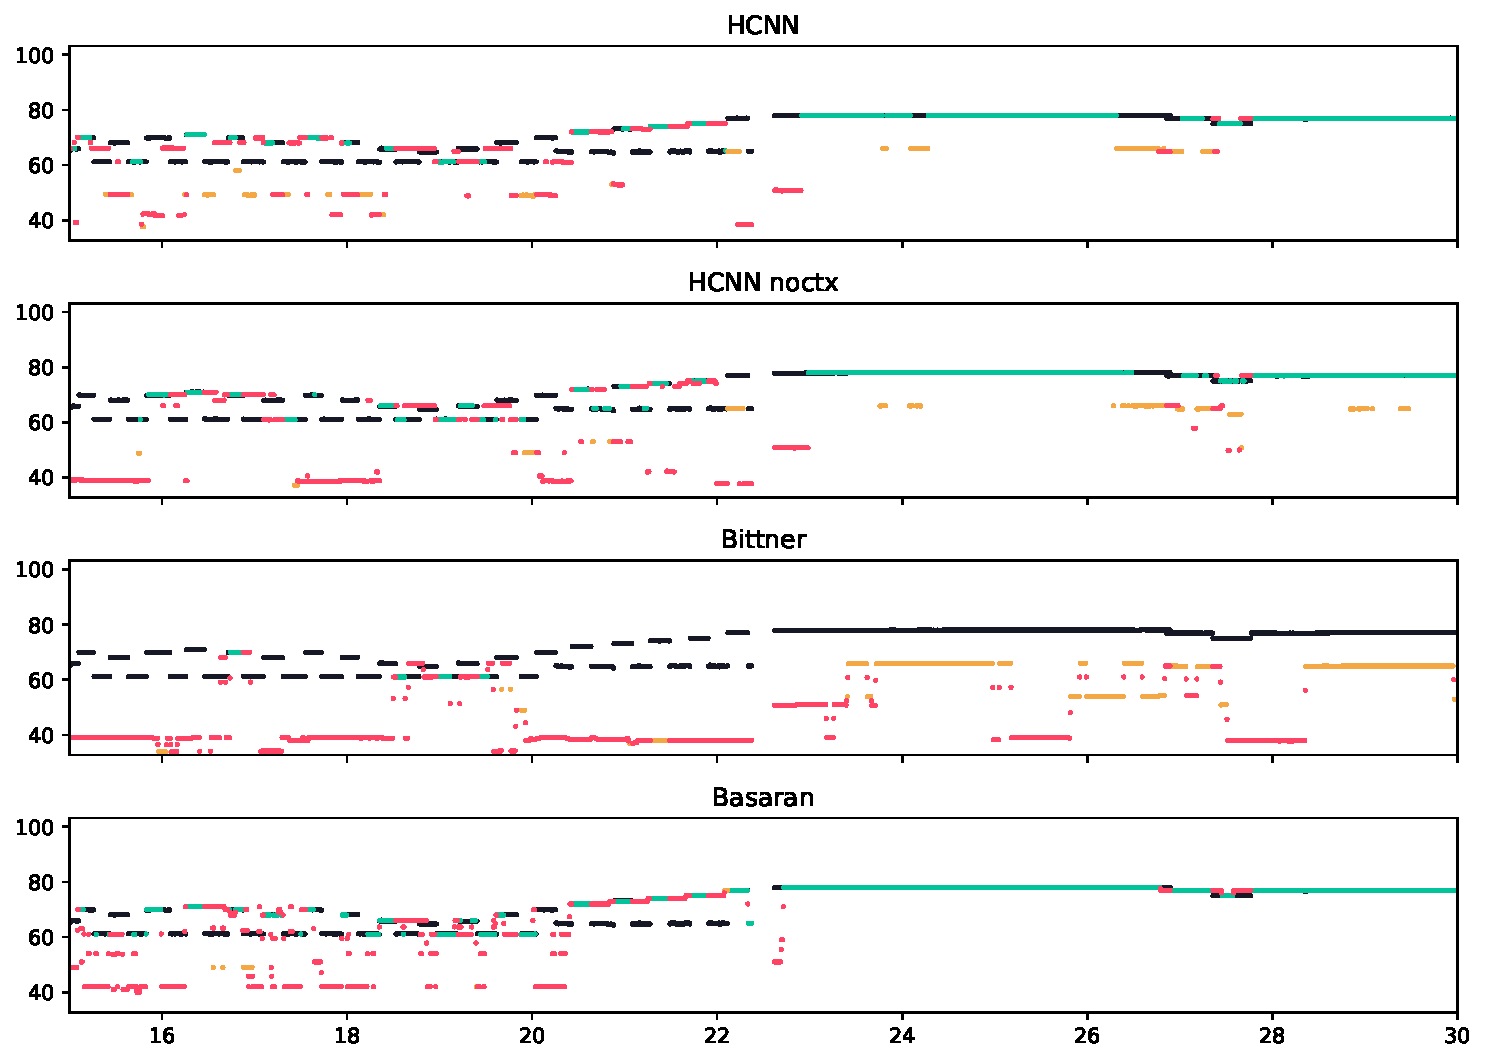
\includegraphics[width=\textwidth,height=\textheight,keepaspectratio]{../img/vysledky/mdb_MatthewEntwistle_FairerHopes}
\caption{Výstup metod na testovacím souboru \texttt{MatthewEntwistle\_FairerHopes} z datasetu MedleyDB.}
\label{obr:mdb_MatthewEntwistle_FairerHopes}
\end{figure}

\begin{table}[h!]
\centering

  \begin{tabular}{ll}
  \toprule
  Metrika (Metoda) & MatthewEntwistle\_FairerHopes \\
  \midrule
        RPA (HCNN) &                        0.451 \\
        RCA (HCNN) &                        0.626 \\
    RPA (Bittner) &                        0.118 \\
    RCA (Bittner) &                        0.423 \\
    RPA (Basaran) &                        0.544 \\
    RCA (Basaran) &                        0.661 \\
  \bottomrule
  \end{tabular}

\caption{Přesnost metod na testovacím souboru \texttt{MatthewEntwistle\_FairerHopes} z datasetu MedleyDB.}\label{tab:mdb_MatthewEntwistle_FairerHopes}
\end{table}




% \begin{figure}[h]\centering
% 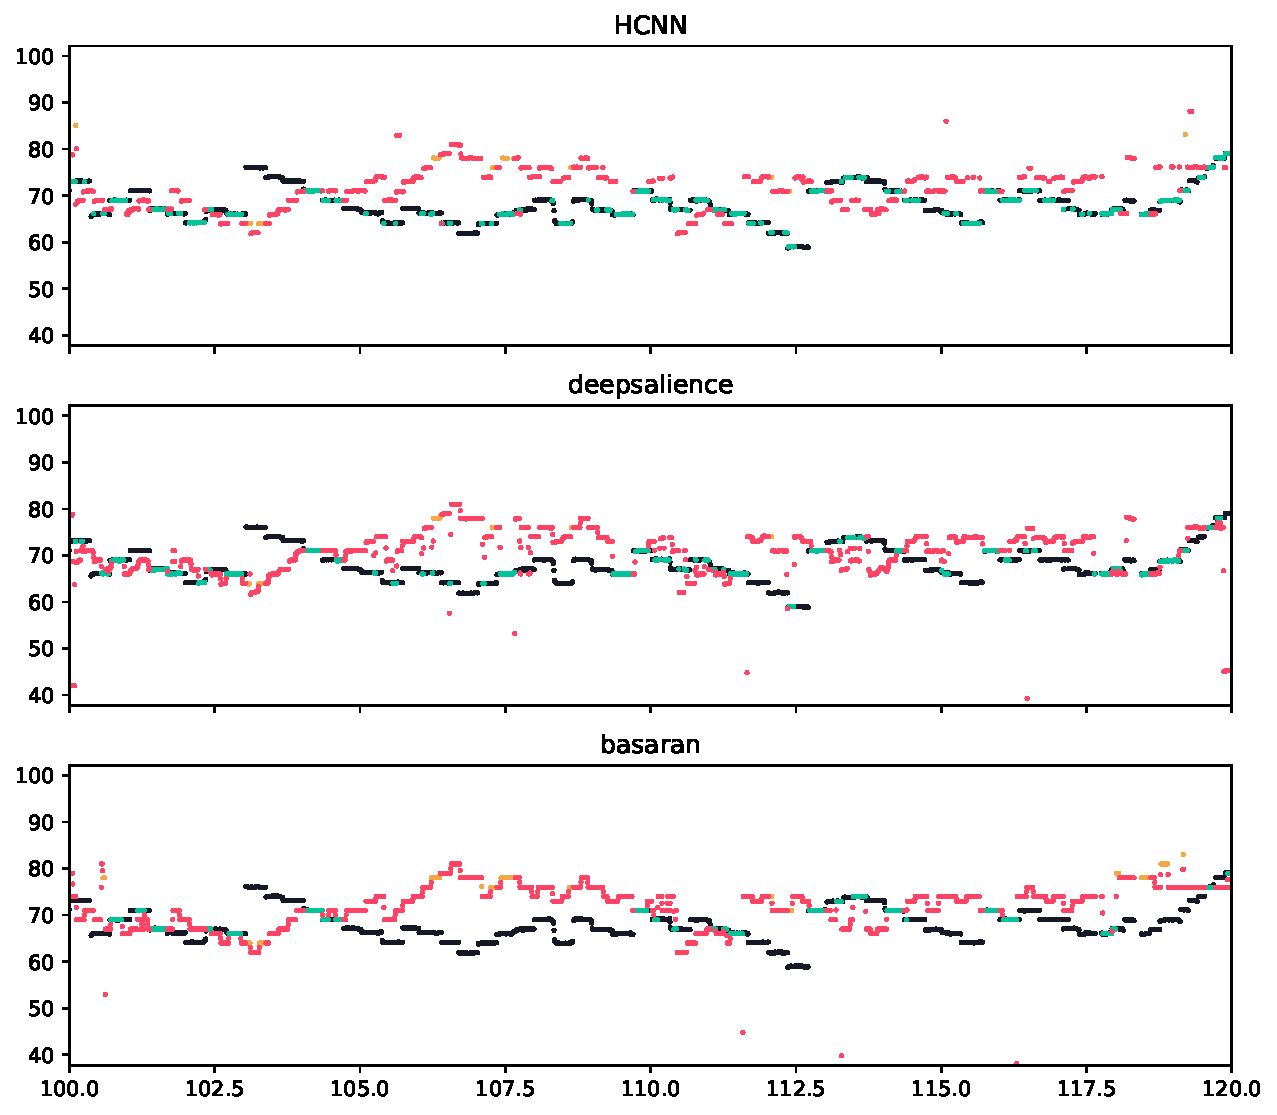
\includegraphics[width=\textwidth,height=\textheight,keepaspectratio]{../img/vysledky/mdb_MusicDelta_Pachelbel}
% \caption{Výstup metod na testovacím souboru \texttt{MusicDelta\_Pachelbel} z datasetu MedleyDB.}
% \label{obr:mdb_MusicDelta_Pachelbel}
% \end{figure}

% \begin{table}[h!]
% \centering

% \begin{tabular}{ll}
% \toprule
% Metrika (Metoda) & MusicDelta\_Pachelbel \\
% \midrule
%       RPA (HCNN) &                0.472 \\
%       RCA (HCNN) &                0.510 \\
%    RPA (Bittner) &                0.461 \\
%    RCA (Bittner) &                0.493 \\
%    RPA (Basaran) &                0.435 \\
%    RCA (Basaran) &                0.491 \\
% \bottomrule
% \end{tabular}

% \caption{Přesnost metod na testovacím souboru \texttt{MusicDelta\_Pachelbel} z datasetu MedleyDB.}\label{tab:mdb_MusicDelta_Pachelbel}
% \end{table}

